% ========================================= TEMPLATE INFO ========================================
%
% Author:       P4ntomime
% Version:      1.0.0
% Last updated: 2024-02-18
% Brief:        A LaTeX template for summaries. See README.md for more information.
% 
% ================================================================================================
\documentclass[8pt, a4paper, twoside, landscape]{extarticle}
% Font size:    8pt
% Paper size:   A4
% style:        twoside (needed, so odd and even pages have different margins)
% orientation:  portrait. (use 'landscape' for landscape orientation)


% ========================================= DOCUMENT INFO =========================================
\def\title{Integraltransformationen}           						% title
\def\shorttitle{IntTra} 											% short title (displayed as PDF title)
\def\dozent{Dr. Manuel Bichsel}         							% lecturer
\def\semester{HS 2022}    	 										% semester
\def\author{Simone Stitz, Luca Loop}        						% author(s)
\def\repo{https://gitlab.com/sstitz/integraltransformationen}       % repository link
\def\version{2.0.\today}    										% version
\def\pagelimit{4}           										% page limit -> causes pages after limit to be red
\def\titleoption{compact}   										% options: compact, normal
\def\enableToC{false}

% ================================= PACKAGES, SETUP AND COMMANDS ==================================
\input{preamble.tex}


% =========================================== DOCUMENT ============================================
\begin{document}
    \begin{layout}
        \section{LTI-Systeme}

Ein LTI-System ist ein System $S$ (Operator), welches eine Funktion $x = x(t)$ auf eine Funktion $y = y(t)$ abbildet und sowohl \textbf{linear}, 
als auch \textbf{zeitinvariant} ist.

\begin{center}
    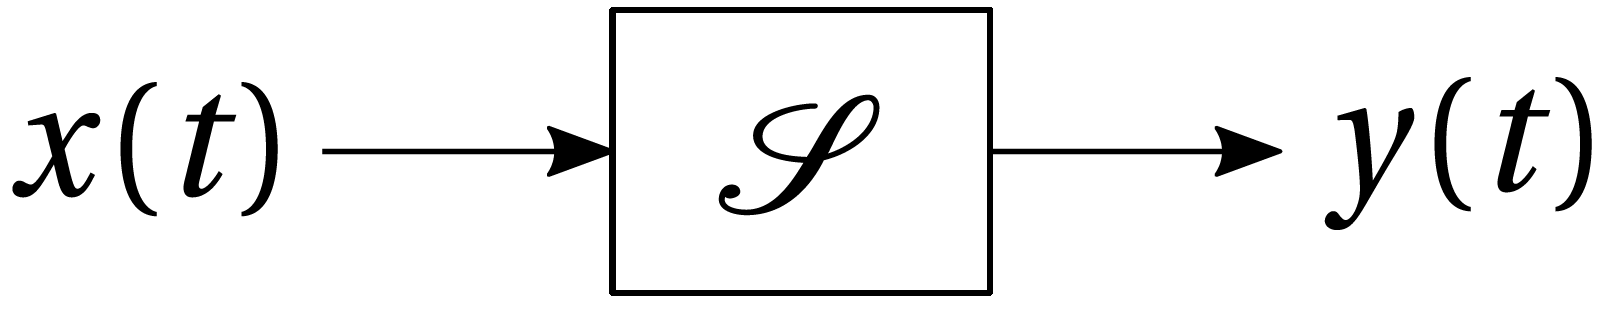
\includegraphics[width=0.7\columnwidth]{images/LTI_system.png}
\end{center}


\begin{tabular}{ll}
    linear          & $S \{ a_1 \cdot x_1(t) + a_2 \cdot x_2(t) \} = a_1 \cdot S \{ x_1(t) \} + a_2 \cdot S \{x_2(t) \}$    \\
                    & für $a,b \in \mathbb{R}$ \qquad (Linearkombination)                                                   \\
    \\
    zeitinvariant   & $S \{ x(t) \} = y(t)$ \textrightarrow\  $S \{ x(t + t_0) \} =  y(t + t_0)$                            \\
                    & für $t_0 \in \mathbb{R}$ \qquad (Zeitverschiebung)                                                    \\
                    & Ein um $t_0$ späteres Eingangssignal bewirkt ein um $t_0$ späteres                                    \\
                    & Ausgangssignal                                                                                        \\
    \\
    Notation        & $S : \, x(t) \mapsto y(t) = S \{x(t) \} = S[x](t)$
\end{tabular}


		\section[Dirac-Funktion (Delta-Funktion)]{Dirac-Funktion (Delta-Funktion) $\bm{\delta = \delta(t)}$}

Die Systemantwort eines LTI-Systems auf eine beliebige Anregung $x = x(t)$ kann bestimmt werden, wenn man die Systemantwort auf die 
Dirac-Funktion kennt (Impulsantwort $y_{\delta} = y_{\delta}(t)$) 


\subsection{Darstellung der Dirac-Funktion}

\begin{center}
    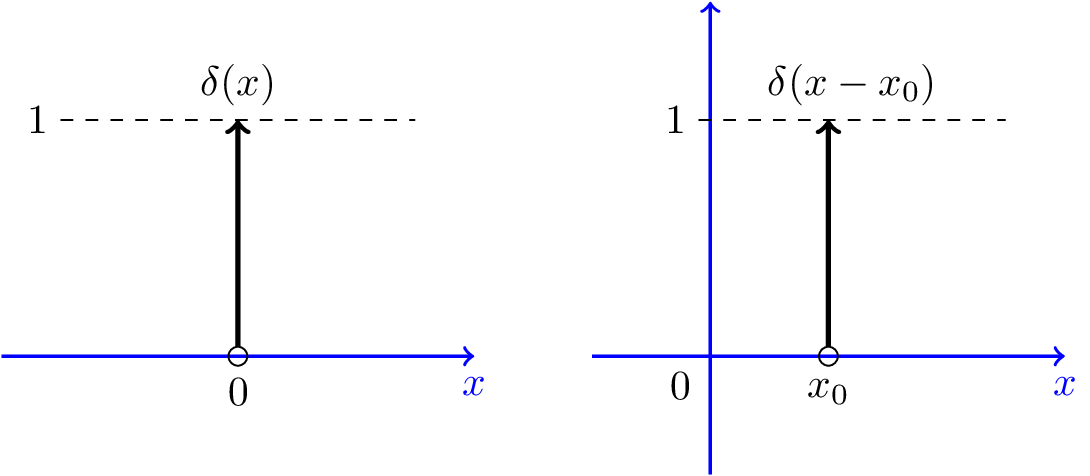
\includegraphics[width=0.7\columnwidth]{images/delta-funktion.png}
\end{center}


\example{Linearkombination mehrerer Dirac-Funktionen}

\vspace{-0.2cm}
$$ 2 \delta(t+1) - \delta(t-2) \qquad \text{ (\textrightarrow\ Ausblendeigenschaft) } $$


\subsection{Eigenschaften der Dirac-Funktion}

\begin{itemize}
    \item Flächeninhalt immer gleich 1 \qquad $\int \limits_{- \infty}^{\infty} \delta(t) \, \diff t = 1$
    \item Unendlich kurzer Impuls \quad $ \delta(t) = 0$ für $t \neq 0$
    \item Für $t = 0$ ist \textbf{kein} Funktionswert definiert; $\neq \infty$
    \item Ausblendeigenschaft (Funktionswerte herausfiltern) \\
        Funktion $f = f(t)$ stetig bei $t = t_0 \in \mathbb{R}$ \qquad  $\int \limits_{- \infty}^{\infty} \delta(t - t_0) \cdot f(t) \, \diff t = f(t_0) $
    \item Dirac-Funktion ist \textbf{verallgemeinerte Ableitung} der (Einheits-) Sprungfunktion \\
        \textrightarrow\ $\delta(t) = \dot{\sigma}(t)$ 
\end{itemize}


		\section{Faltungsprodukt}

Bei LTI-Systemen wird das Faltungsprodukt benötigt, um aus der Impulsantwort  $y_{\delta} = y_{\delta}(t)$ und der Anregungsfunktion 
$x = x(t)$ das Ausgangssignal $y = y(t)$ zu berechnen.


\subsection{Definition des Faltungsprodukts}

\renewcommand{\arraystretch}{2}
\begin{tabular}{ll}
    Allgemein:  & $ (f * g)(t) = \int\limits_{-\infty}^{\infty} f(\tau) \cdot g(t - \tau) \, \diff \tau$                            \\
    LTI-System: & $y(t) = (x * y_{\delta} )(t) = \int \limits_{-\infty}^{\infty} x(\tau) \cdot y_{\delta}(t - \tau) \, \diff \tau $ 
\end{tabular}
\renewcommand{\arraystretch}{1}


\subsection{Eigenschaften des Faltungsprodukts} 

\begin{itemize}
    \item Faltungsprodukt ist kommutativ \textrightarrow\ $(f * g)(t) = (g * f)(t)$
    \item Dirac-Funktion $\delta(t)$ als neutrales Element \\   
        $\delta(t - t_0) * f(t) = f(t) * \delta(t - t_0) = f(t - t_0)$
\end{itemize}


\subsection{Bestimmung des Faltungsprodukts}

\example{Grafische Bestimmung des Faltungsprodukts}

Die Funktion $g(t - \tau)$ (entspricht der an der $y$-Achse gespiegelten Funktion $g(t)$) wird über die Funktion $f(t)$ geschoben. 
Das \textbf{Produkt} der Funktionswerte \textbf{zu jedem Zeitpunkt} $t$ ergibt das Faltungsprodukt.


\begin{minipage}{0.45\columnwidth}
    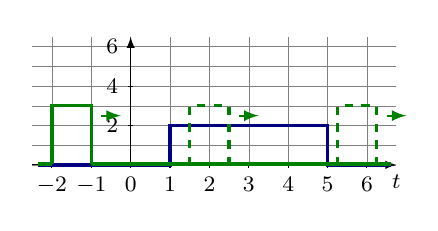
\begin{tikzpicture}
    [
    x=1cm, y=0.5cm, scale=0.5, font=\footnotesize, >=latex 
    %Voreinstellung für Pfeilspitzen
    ]
    
    %Raster im Hintergrund
    \draw[step=1, gray, very thin] (-2.5,0) grid (6.75,6.5);
    
    %Zahlen auf x-Achse
    \foreach \x in {-2,-1,0,1,2,3,4,5,6}
    \draw[shift={(\x,0)},color=black] (0pt,2pt) -- (0pt,-2pt) node[below]
    {\footnotesize $\x$};
    
    %Länge x Achse
    \draw [-latex] (-2.5,0) -- ++(9.25,0) node[below] {$t$};
    
    %Länge y Achse
    \draw [-latex] (0,0) -- ++(0,6.5) node[left] {$ $};
    
    %Zahlen auf y-Achse 
    %\foreach \y in {0,...,1}
    \foreach \y in {2,4,6}
    \draw[shift={(0,\y)},color=black] (2pt,0pt) -- (-2pt,0pt) node[left]
    {\footnotesize $\y$};		
    
    %f(t)
    \draw[blue!50!black, very thick] (-2.35,0) -- (1,0) -- (1,2) -- (5,2) -- (5,0) -- (6.6,0); 
    
    %g(t)
    \draw[green!50!black, very thick] (-2,0.05) -- (-2,3) -- (-1,3) -- (-1,0.05); 
    \draw[-latex,green!50!black, thick] (-0.75,2.5) -- (-0.25,2.5);
    
    \draw[green!50!black, very thick] (-2.35,0.05) -- (-2,0.05); 
    \draw[green!50!black, very thick] (-1,0.05) -- (6.6,0.05);		
    
    \draw[dashed, green!50!black, very thick] (1.5,0) -- (1.5,3) -- (2.5,3) -- (2.5,0); 
    \draw[-latex,green!50!black, thick] (2.75,2.5) -- (3.25,2.5);
    
    \draw[dashed, green!50!black, very thick] (5.25,0) -- (5.25,3) -- (6.25,3) -- (6.25,0); 
    \draw[-latex,green!50!black, thick] (6.5,2.5) -- (7,2.5);		
        
    
    %Vektor a
    %\draw[-latex, thick] (0,0) -- (2,3) node [midway, above] {$\vec{a}$} node (a) {}; 
    %Vektor b
    %\draw[-latex, thick] (0,0) -- (3,0) node [midway, above] {$\vec{b}$} node (b) {}; 
    %\draw[dashed] (a.center) -- ++ (3,0) node (c) {};
    %\draw[dashed] (b.center) -- ++ (2,3);
    %\draw[very thick, red, -latex] (0,0) -- (c.center) node [midway, above] {$\vec{c}$};
\end{tikzpicture}
\end{minipage}
\hfill
\begin{minipage}{0.45\columnwidth}
    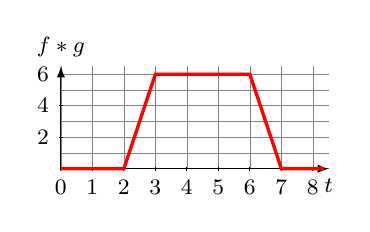
\begin{tikzpicture}
    [
    x=1cm, y=0.5cm, scale=0.4, font=\footnotesize, >=latex 
    %Voreinstellung für Pfeilspitzen
    ]
    
    %Raster im Hintergrund
    \draw[step=1, gray, very thin] (0,0) grid (8.5,6.5);
    
    %Zahlen auf x-Achse
    \foreach \x in {0,1,2,3,4,5,6,7,8}
    \draw[shift={(\x,0)},color=black] (0pt,2pt) -- (0pt,-2pt) node[below]
    {\footnotesize $\x$};
    
    %Länge x Achse
    \draw [-latex] (0,0) -- ++(8.5,0) node[below] {$t$};
    
    %Länge y Achse
    \draw [-latex] (0,0) -- ++(0,6.5) node[above] {$f*g$};
    
    %Zahlen auf y-Achse 
    %\foreach \y in {0,...,1}
    \foreach \y in {2,4,6}
    \draw[shift={(0,\y)},color=black] (2pt,0pt) -- (-2pt,0pt) node[left]
    {\footnotesize $\y$};
    
    %f(t)
    \draw[red, very thick] (0,0) -- (2,0) -- (3,6) -- (6,6) -- (7,0) -- (8.35,0); 
\end{tikzpicture}
\end{minipage}


\example{Rechnerische bestimmung des Faltungsprodukts}

\textbf{WICHTIG: Immer die einfacher definierte Funktion als $\bm{g(t - \tau)}$ wählen!} \\
(\textrightarrow\ kommutativ)

\vspace{0.2cm}

\begin{minipage}[t]{0.45\columnwidth}
    $f(t) = \begin{cases}
    2 & \text{für } \, 0 < t < 4 \\
    0 & \text{sonst}
    \end{cases}$  
\end{minipage}
\hfill
\begin{minipage}[t]{0.5\columnwidth}
    $g(t) = \begin{cases}			
    3 & \text{für } \, 0 < t < 1 \\
    0 & \text{sonst}
    \end{cases}$  	
\end{minipage}

\vspace{0.2cm}

\begin{enumerate}
    \setlength{\itemsep}{5pt} % adjust space between items

    \item \textbf{Variablentransformation}
    
    \vspace{0.2cm}

    \begin{minipage}[t]{0.45\columnwidth}
        $f(\tau) = \begin{cases}			
        2 & \text{für } \, 0 < \tau < 4 \\
        0 & \text{sonst}
        \end{cases}$ 
    \end{minipage}
    \hfill
    \begin{minipage}[t]{0.5\columnwidth}
        $g(t - \tau) = \begin{cases}			
        3 & \text{für } \, 0 < t - \tau < 1 \\
        0 & \text{sonst}
        \end{cases}$ 
    \end{minipage}

    \item  \textbf{Nach $\bm{\tau}$ auflösen (speziell bei $\bm{g(t - \tau)}$)}
        $$ 0 < t - \tau < 1 \quad \text{ \textrightarrow\ } \quad 0 - t < - \tau < 1 - t  \quad \text{ \textrightarrow\ } \quad \cgn{t} > \tau > \cgn{t - 1} $$

    \item \textbf{Hilfsdiagramm zeichnen}
    \begin{center}
        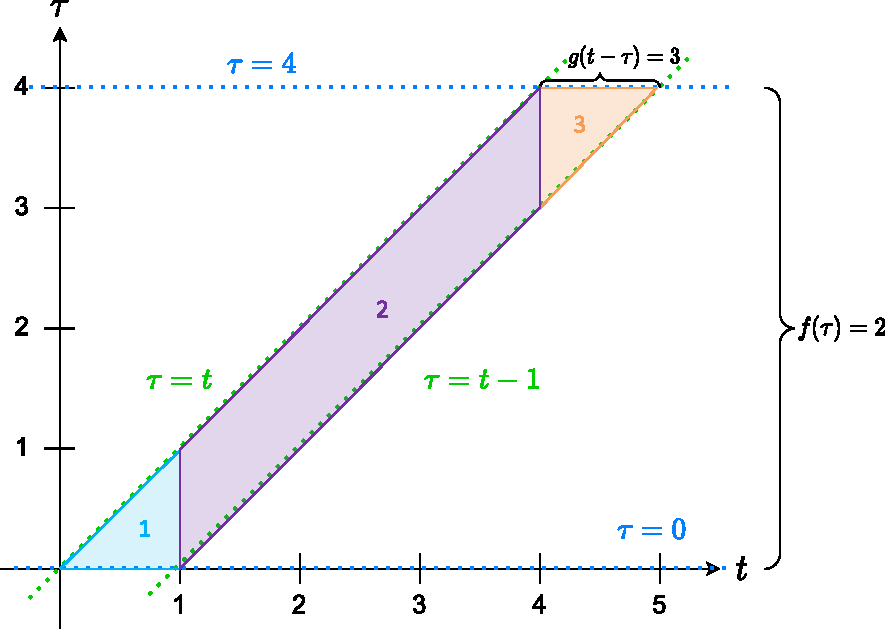
\includegraphics[width=0.85\columnwidth]{images/hilfsdiagramm.pdf}
    \end{center}
    
    \columnbreak

    \item \textbf{Faltungsprodukt abschnittweise berechnen}

    \renewcommand{\arraystretch}{2.5}
        \begin{tabular}{ll}
            $0 \leq t < 1$  & $(f * g)(t) = \int\limits_0^t 2 \cdot 3 \, \diff \tau$         \\
            $1 \leq t < 4$  & $(f * g)(t) = \int\limits_{t-1}^t 2 \cdot 3 \, \diff \tau$     \\
            $4 \leq t < 5$  & $(f * g)(t) = \int\limits_{t-1}^4 2 \cdot 3 \, \diff \tau$     \\
            sonst           & $(f * g)(t) = 0$
        \end{tabular}
    \renewcommand{\arraystretch}{1}
\end{enumerate}


		\section{Fouriertransformation}

Die Fouriertransformation führt eine Funktion vom Zeitbereich in den Frequenzbereich über. Die Rücktransfomration 
(inverse Fouriertransformation) macht dies wieder rückgängig.

\begin{center}
    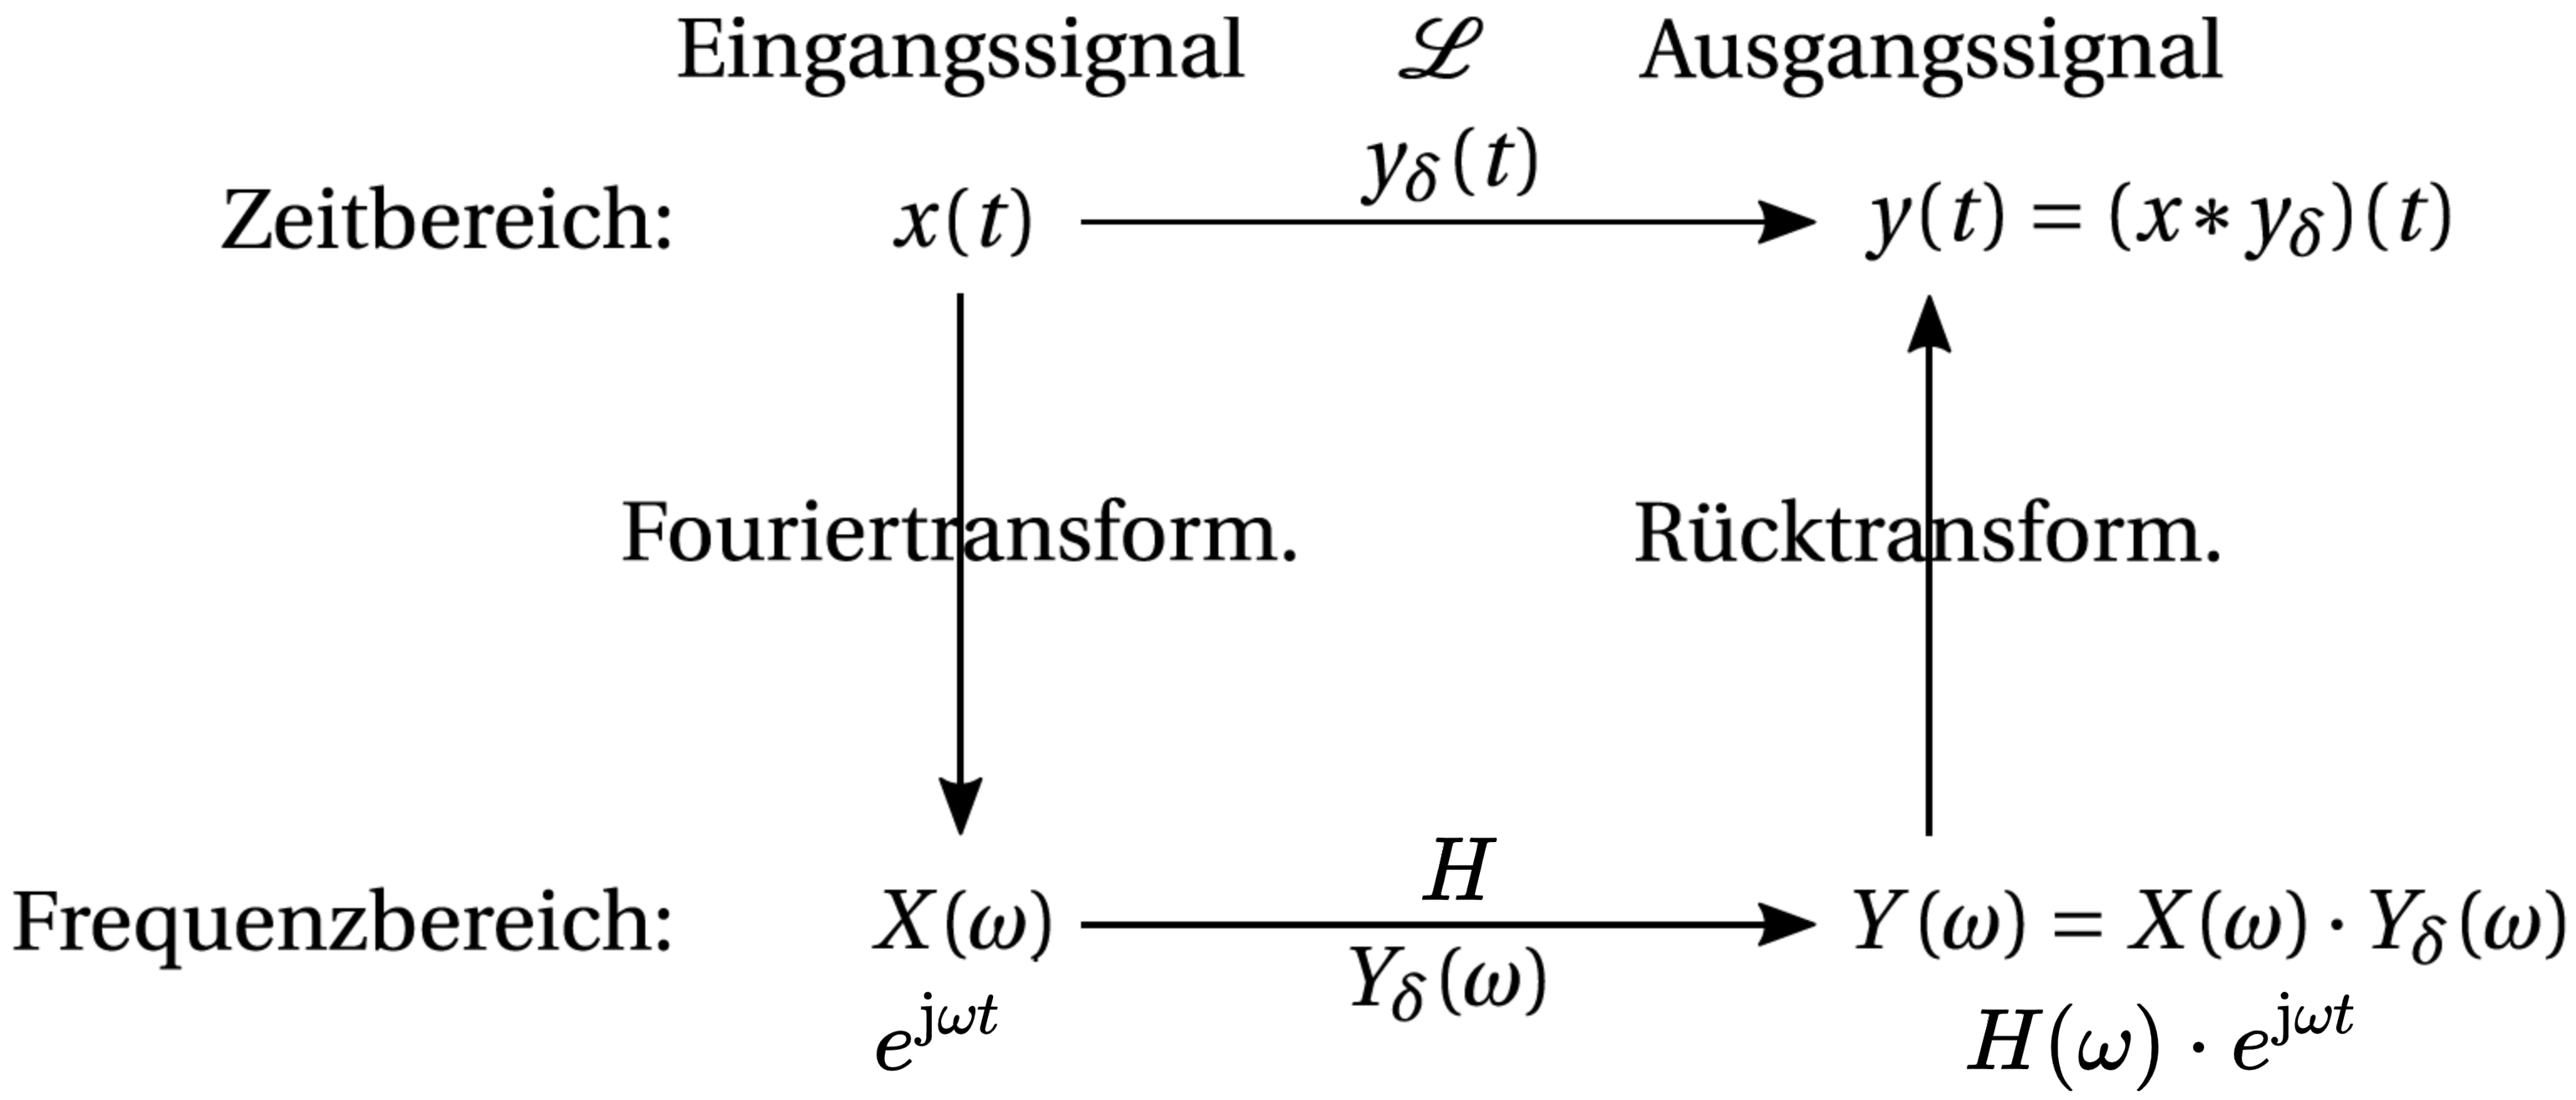
\includegraphics[width=0.7\columnwidth]{images/zeitbereich_frequenzbereich.png}
\end{center}

\vspace{-0.2cm}


\subsection{Komplexe trigonometrische Funktionen} 

\begin{tabular}{lll}
    $\sin(\omega t) = \frac{\e^{\jimg\omega t} - \e^{-\jimg \omega t}}{2\jimg}$ &
    $\cos(\omega t) = \frac{\e^{\jimg \omega t} + \e^{-\jimg \omega t}}{2}$ & 
    $\tan(\omega t) = \frac{\sin(\omega t)}{\cos(\omega t)}$
\end{tabular}


\subsection{Frequenzgang (Frequenzerhaltung)}

Der Frequenzgang $H(\omega)$ bestimmt die Änderung von Amplitude und Phase des Eingangssignals.

\textbf{Amplitudengang:} $ A(\omega) = \left|H(\omega)\right| = \sqrt{H(\omega) \cdot \overline{H(\omega)}} = \sqrt{\Re(H(\omega))^2 + \Im(H(\omega))^2}$

\vspace{0.2cm}

\textbf{Phasengang:} $\Phi(\omega) = \arg(H(\omega)) = \begin{cases}
\arccos\left(\frac{ \Re(H(\omega))}{|H(\omega)|}\right)  & \text{für} \; \Im(H(\omega)) \geq 0 \\
-\arccos\left(\frac{ \Re(H(\omega))}{|H(\omega)|}\right) & \text{für} \; \Im(H(\omega)) < 0
\end{cases}$

\vspace{0.2cm}

\begin{tabular}{ll}
    Amplitudengang: & achsensymmetrisch (gerade)    \\
    Phasengang:     & punktsymmetrisch (ungerade)
\end{tabular}


\subsection{Systemantwort berechnen}

Die Systemantwort $y(t)$ (Ausgangssignal) auf ein \cbl{Eingangssignal $x(t)$} berechnet sich mit dem Frequenzgang $H(\omega)$ 
$$ y(t) = H(\omega) \cdot \cbl{x(t)} \qquad \qquad \mathcal{L} \{ \cbl{ \e^{\jimg \omega  t} } \} = H(\omega) \cdot \e^{\jimg \omega t} $$ 


\example{Systemantwort $y(t)$ berechnen}

\vspace{-0.2cm}
$$\cbl{x(t) = \sin(2t)} \qquad H(2) = \frac{-3-2\jimg}{13} \qquad H(-2) = \frac{-3+2\jimg}{13}$$
\vspace{-0.4cm}

\begin{align*}
    y(t)    &= \mathcal{L} \Big\{ \frac{1}{2 \jimg}  \left( \e^{\jimg 2t} - \e^{- \jimg 2t} \right) \Big\} = \frac{1}{2 \jimg} \left(H(2) \cdot \e^{\jimg 2t} - H(-2) \cdot \e^{-\jimg 2t} \right) \\
            &= \frac{1}{2\jimg} \left( \frac{-3-2\jimg}{13} \cdot \e^{\jimg2t} - \frac{-3+2\jimg}{13} \cdot \e^{-\jimg2t} \right) \\
            &= -\frac{3}{13} \underbrace{ \frac{1}{2\jimg} \left( \e^{\jimg2t} - \e^{-\jimg2t} \right)}_{\substack{\sin(2t)}} + \frac{-2 \jimg}{13}  \frac{1}{ \jimg} \underbrace{ \frac{1}{2} \left( \e^{\jimg2t} + \e^{-\jimg2t} \right)}_{\substack{\cos(2t)}}
\end{align*}

\begin{itemize}
    \item Realteil und Imaginärteil \textbf{getrennt} ausklammern! \\
        \textbf{Hinweis:} Wenn $x(t)$ und $y(t)$ bekannt sind, $H(\omega)$ allerdings nur mit Parametern gegeben ist, dann wird mit Ansatz
        $y(t) = H(\omega) \cdot x(t)$ mit Parametern gerechnet
    \item Mit Koeffizientenvergleich fehlende Parameter bestimmen
\end{itemize}


\subsection{Berechnung der Fouriertransformation}

Wenn eine Funktion $f(t)$ im Zeitbereich absolut integrierbar ist, d.h. $\int \limits_{-\infty}^{\infty} | f(t) | \,  \diff t < \infty$, 
dann funktioniert die Umwandlung:

\renewcommand{\arraystretch}{2.5}
\begin{tabular}{ll}
    Fouriertransformierte:  & $F(\omega) = \int \limits_{-\infty}^{\infty} f(t) \, \e^{- \jimg \omega t} \, \diff t$                    \\
    Rücktransformation:     & $f(t) = \frac{1}{2 \pi} \int \limits_{-\infty}^{\infty} F(\omega) \, \e^{\jimg \omega t} \, \diff \omega$
\end{tabular}
\renewcommand{\arraystretch}{1}


\subsubsection{Darstellung der Fouriertransformierten}

\begin{tabular}{ll}
    Spektraldichte:     & entspricht der Fouriertransformierten $F(\omega)$     \\
                        & Die komplexwertige Funktion wird für die Darstellung  \\ 		    
                        & aufgeteilt in Folgendes: \\
    \\
    Amplitudendichte:   & $\vert F(\omega) \vert$ \quad (Betrag der Fouriertransformierten)     \\
    Phasendichte:       &  $\mathrm{arg}( F(\omega))$ \quad (Winkel der Fouriertransformierten)
\end{tabular}


\subsection{Eigenschaften / Rechenregeln Fouriertransformation}

\textbf{\textrightarrow\ siehe Tabelle!}

\textbf{Es folgen Ergänzungen zur Tabelle}	


\subsubsection{Sprungstellen / Symmetrie}

\begin{itemize}
    \item An allfälligen \textbf{Sprungstellen} von $f(t)$ konvergiert die Rücktransformierte von $F(\omega)$ gegen die 
        \textbf{Mitte} der Sprungstelle
    \item Ist $f(t)$ \textbf{gerade}, so hat $F(\omega)$ nur \textbf{reelle} Funktionwerte
    \item Ist $f(t)$ \textbf{ungerade}, so hat $F(\omega)$ nur \textbf{imaginäre} Funktionwerte
\end{itemize}


\subsubsection{Vertauschungssatz; Zeit-Frequenz-Symmetrie}

Ist $f(t) \; \laplace \; F(\omega)$ ein Korrespondenzpaar, dann ist auch $F(t) \; \laplace \; 2 \pi f(-\omega)$ ein Korrespondenzpaar.


\subsubsection{Satz von Parseval / Plancherel}
Ist $F(\omega)$ die Fouriertransformierte von $f(t)$, so gilt

$\int \limits_{-\infty}^{\infty} \vert f(t) \vert ^2 \, \diff t
= \frac{1}{2 \pi} \int \limits_{-\infty}^{\infty} \vert F(\omega) \vert ^2 \, \diff \omega $
, falls $\int \limits_{-\infty}^{\infty} \vert f(t) \vert ^2 \, \diff t$ existiert


\subsection{Wichtige Korrespondenzpaare}

\renewcommand{\arraystretch}{1.5}
\begin{tabular}{r c l}
    $\cos(\omega_0 \, t)$   & $\laplace$    & $\pi(\delta( \omega + \omega_0) + \delta ( \omega - \omega_0))$       \\
    $\sin(\omega_0 \, t)$   & $\laplace$    & $\jimg \pi(\delta( \omega + \omega_0) - \delta ( \omega - \omega_0))$
\end{tabular}
\renewcommand{\arraystretch}{1}


\subsection{Fouriertransformierte einer Fourierreihe}

\vspace{-0.2cm}
$$ f(t) = \sum \limits_{k = - \infty}^{\infty} c_k \, \e^{\jimg k \omega_0 t} \;  \laplace \; 
F(\omega) = 2 \pi \sum \limits_{k = - \infty}^{\infty} c_k \, \delta(\omega - k \omega_0) $$


\subsection{Sampling zeitlich kontinuierlicher Signale}

Mathematisch wird das abzutastende Signal $x(t)$ mit einem \textbf{Dirac-Kamm $\bm{\delta_T(t)}$} multipliziert.
$$ \text{Dirac-Kamm:} \quad \delta_T(t) = \sum \limits_{n = - \infty}^{\infty} \delta(t - nT)$$

Es resultiert das abgetastete Signal $x_a (t)$
$$ x_a (t) = \sum \limits_{n = - \infty}^{\infty} x(t) \cdot \delta(t - nT) = \sum \limits_{n = - \infty}^{\infty} \underbrace{x(nT)}_{\substack{x[n]}} \cdot \delta(t - nT) $$

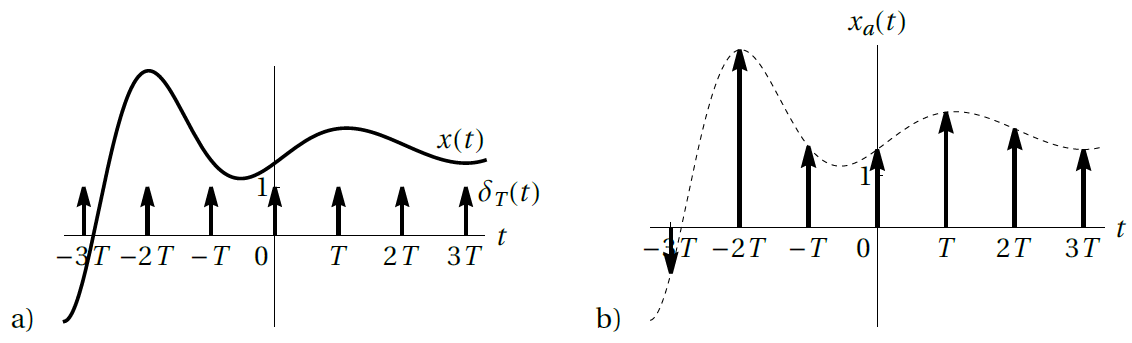
\includegraphics[width=\columnwidth]{images/sampling.png}

\vspace{0.2cm}

\textbf{Wechsel in den Frequenzbereich (Fouriertransformierte)}
$$ x_a (t) = \sum \limits_{n = - \infty}^{\infty} x[n]\cdot \delta(t - nT)  \; \laplace \; 
X_a(\omega) = \frac{1}{T} \sum \limits_{n = - \infty}^{\infty} X(\omega - n \omega_a) \quad \text{mit } \omega_a = \frac{2 \pi}{T} $$		 


\subsection{Diskrete Fouriertransformation (DFT)}

$x[n]$ ist für $n \in \{ 0, \, ... \, , N-1 \} $ eine endliche Folge von reellen Zahlen

\vspace{0.2cm}

\renewcommand{\arraystretch}{2.8}
\begin{tabular}{ll}
    $x[n] = \sum \limits_{k = 0}^{N-1} c_k \, e^{\jimg k (2 \pi / N) \, n}$                 & für $n \in \{ 0, \, \ldots \, , N-1 \}$ \\
    $c_k = \frac{1}{N} \sum \limits_{n = 0}^{N-1} x[n] \, e^{- \jimg k (2 \pi / N) \, n}  $ & für $k \in \{ 0, \, \ldots \, , N-1 \}$ 
\end{tabular}				
\renewcommand{\arraystretch}{1}


\example{Abtastwerte $x[n]$ finden}

\begin{minipage}[c]{0.55\columnwidth}
    Ein Signal $s(t)$ wird auf dem Intervall [0,1] mit der Frequenz $f_a = 4 \, \text{Hz}$ abgetastet.
\end{minipage}
\hfill
\begin{minipage}[c]{0.38\columnwidth}
    $s(t) = \begin{cases}			
        t(1-t)  & \text{für} \; t \in [0,1] \\
        0       & \text{sonst} 
    \end{cases}$  
\end{minipage}

\vspace{0.2cm}

\renewcommand{\arraystretch}{2}
\begin{tabular}{lll}
    $x[0] = s(0) = 0$                                                                               & & 
    $x[1] = s\left( \frac{1}{4} \right) = \frac{1}{4} \left( 1 - \frac{1}{4} \right) = \frac{3}{16}$    \\
    $x[2] = s \left( \frac{1}{2} \right) = \frac{1}{2} \left(1- \frac{1}{2} \right) = \frac{1}{4}$  & &
    $x[3] = s \left( \frac{3}{4} \right) = \frac{3}{4} \left (1 - \frac{3}{4} \right) = \frac{3}{16}$
\end{tabular}
\renewcommand{\arraystretch}{1}


\subsection{Schnelle Fouriertransformation (FFT)}

\textbf{Bedingung:} Die Länge $N$ der endlichen Folge $x[0], \, \ldots \, , x[N-1]$ muss einer Zweierpotenz entsprechen! 
\textrightarrow\ $N = 2^p \; \text{ mit } \; p \in \mathbb{N}$


\subsubsection{Fourierkoeffizienten $c_k$ für $k < \frac{N}{2}$}

\vspace{-0.2cm}

\renewcommand{\arraystretch}{2.5}
\begin{tabular}{ll}
    $c_k = \frac{1}{N} \left( c_{g,k} + E_N^k \, c_{u,k} \right)$   & mit $E_N := e^{-\jimg(2 \pi/N)}$  \\
    $c_{g,k}:= \sum \limits_{m = 0}^{N/2-1} x[2m] \,  E_N^{k2m}$    & $c_{u,k}:= \sum \limits_{m = 0}^{N/2-1} x[2m+1] \,  E_N^{k2m}$
\end{tabular}


\subsubsection{Fourierkoeffizienten $c_{k + N/2}$ }

\vspace{-0.2cm}
\begin{tabular}{l}
    $c_{k + N/2} =  \frac{1}{N} \left( c_{g,k} - E_N^k \, c_{u,k} \right)$
\end{tabular}
\renewcommand{\arraystretch}{1}

\columnbreak


		\section{Laplacetransformation}

Laplacetransformationen werden für kausale Funktionen $f(t)$ definiert, für die gilt $f(t) = 0$ für $t < 0$

\vspace{0.1cm}

Es gilt die Korrespondenz: $f(t) \; \laplace \; F(s)$ (Bildbereich)

\vspace{0.1cm}

\textbf{Hinweis:} Eine Funktion kann kausal gemacht werden, indem man sie mit der Einheitssprungfunktion $\sigma(t)$ multipliziert.


\subsection{Berechnung (einseitige) Laplacetransformation}

\renewcommand{\arraystretch}{1.8}
\begin{tabular}{ll}
    Transformation:     & $F(s) = \mathcal{L} \{ f(t) \} := \int \limits_0^{\infty} f(t) \cdot \e^{-s \, t} \, \diff t$ \quad mit $s = \rho + \jimg \omega$   \\
    Rücktransformation: & \textrightarrow\ Tabellen und Tipps verwenden! 
\end{tabular}
\renewcommand{\arraystretch}{1}


\subsection{Konvergenzhalbebene}

Es gibt jeweils mehrere (komplexe) Zahlen $s$, \textbf{für welche das Laplace-Integral konvergiert.} 
Die Konvergenzhalbebene beinhaltet alle diese Zahlen $s$

\begin{minipage}[c]{0.48\columnwidth}
    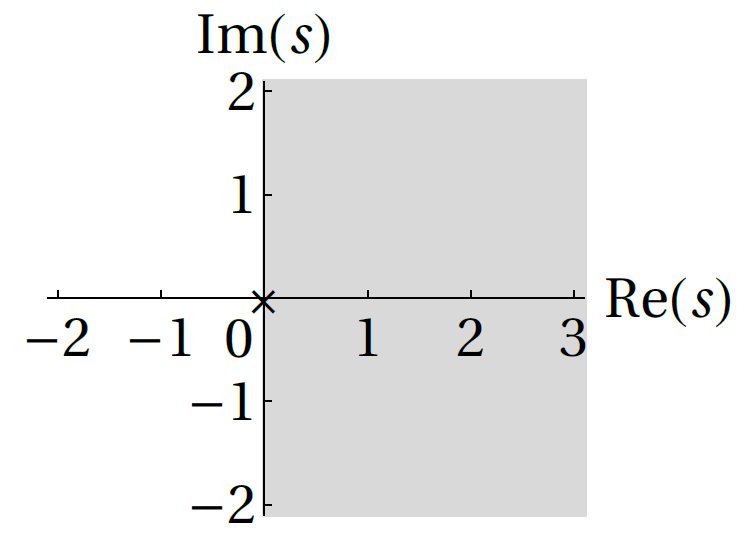
\includegraphics[width=\columnwidth]{images/konvergenzhalbebene} 
\end{minipage}
\hfill
\begin{minipage}[c]{0.48\columnwidth}
    Die Halbebene wird durch die \textbf{am weitesten rechts liegende Polstelle} von $F(s)$ begrenzt (Kreuzchen)
    \vspace{0.2cm}
    Falls $F(s)$ keine Polstelle hat, ist die Konvergenzhalbebene gleich $\mathbb{C}$
\end{minipage}


Liegt die imaginäre Achse in der Konvergenzhalbebene, so \textbf{existiert} die Fouriertransformierte!

\textrightarrow\ Man erhält sie, indem man $s$ durch $\jimg \omega$ ersetzt


\example{Berechnung der Laplacetransformation}

$f(t) = \begin{cases}			
    0           & \text{für} \; t < 0 \\
    \frac{1}{2} & \text{für} \; t = 0 \\ 
    e^{at}      & \text{für} \; t > 0 
\end{cases}$  \quad  mit $a \in \mathbb{R}$

\begin{align*}
    F(s)    &= \int \limits_0^{\infty} \e^{at} \, \e^{-st} \, \diff t = \int \limits_0^{\infty} \e^{-(s-a)t} \, \diff t = - \frac{1}{s-a} \e^{-(s-a)t} \biggr|_0^{\infty} \\
            &= - \frac{1}{s-a} \left( \lim \limits_{t \to \infty} \e^{-(s-a)t} -1 \right) = - \frac{1}{s-a} \left( \lim \limits_{t \to\infty} \e^{-((\rho+ \jimg \omega)-a)t} -1 \right) \\
            &= - \frac{1}{s-a} \left( \lim \limits_{t \to \infty} \e^{-(\rho-a)t} \, \e^{- \jimg \omega t} -1 \right)
\end{align*}

\textrightarrow\ Überlegen, was mit welchem Teil passiert! 

\vspace{0.2cm}

\begin{tabular}{ll}
    $\e^{- j \omega t}$ & Zahl auf Einheitskreis (Betrag 1) \\
    $\e^{-(\rho - a)t}$ & $\rho > a$ \quad \textcolor{blue}{Konvergenz gegen 0} \\
                        & $\rho = a$ \quad Konvergenz gegen 1 \\
                        & $\rho < a$ \quad Divergenz \\
\end{tabular}

\vspace{0.2cm}
$$ F(s) = ... = - \frac{1}{s-a} \left( \lim \limits_{t \to \infty} \e^{-(s-a)t} -1 \right) = \frac{1}{s-a} \text{ für } \rho = \Re(s) > a $$

$$ \text{ \textrightarrow\ Korrespondenzpaar: } \e^{at} \; \laplace \; \frac{1}{s-a} $$


\subsection{Tipps zu Rücktransformationen}

\begin{itemize}
    \item Zähler und Nenner gleichgradig \textrightarrow\ Polynomdivision
    \item Zusammengesetzte Nennerfunktion \textrightarrow\ PBZ
    \item Nenner \textbf{keine} reelle NS \textrightarrow\ Ansatz $ \sin(\omega t), \, \cos(\omega t)$
    \item Nenner hat reelle NS \textrightarrow\ Ansatz \textbf{nicht} $\sin(\omega t), \, \cos(\omega t)$
\end{itemize}


\subsection{Lineare DGL mittels Laplacetransformation lösen}

\subsubsection{Vorgehen: Lösen einer DGL mit Laplace}

\begin{enumerate}
    \item DGL inkl. Störfunktion $f(t)$ in Bildbereich transformieren \\
        \textrightarrow\ Anfangswerte für $f^{(n)}(0^+)$ einsetzen!
    \item Gleichung nach Laplace-Transofrmierter der gesuchten Funktion umformen
    \item Rücktransformation in den Zeitbereich
\end{enumerate}


\example{Lösung einer DGL mit Laplace}

\begin{minipage}[c]{0.6\columnwidth}
    \begin{tabular}{ll}
        DGL:            & $\ddot{y}(t) + 2 \, \dot{y}(t) + 5 \, y(t) = f(t)$ \\
        Anfangswerte:   & $y(0) = 0$; \quad $\dot{y}(0) = 0$
    \end{tabular}
\end{minipage}
\hfill
\begin{minipage}[c]{0.35\columnwidth}
    \textrightarrow\ Finde $y(t)$
\end{minipage}

\vspace{0.2cm}

\begin{enumerate}
    \setlength\itemsep{3pt}
    \item $\laplace \; s^2 \cdot Y(s) - s \cdot 0 - 0 + 2( s \cdot Y(s) - 0) + 5 \cdot Y(s) = 1(s)$ \\
        $s^2 \cdot Y(s)+ 2 \cdot s \cdot Y(s) + 5 \cdot Y(s) = 1(s)$
    \item $Y(s) = \frac{1}{s^2 + 2s +5}$
    \item Rücktransformation mit Tabellen
\end{enumerate}


\subsection[Übertragungsfunktion (LTI-Systeme)]{Übertragungsfunktion $\bm{G(s)}$ (LTI-Systeme)}

\begin{minipage}[c]{0.4\columnwidth}
    $$ G(s) = Y_{\delta}(s) = \frac{Y(s)}{X(s)} $$
\end{minipage}
\hfill
\begin{minipage}[c]{0.58\columnwidth}
    \begin{tabular}{ll}
        Eingangssignal: & $x(t) \; \laplace \; X(s)$    \\
        Ausgangssignal: & $y(t) \; \laplace \; Y(s)$
    \end{tabular}
\end{minipage}

\begin{center}
    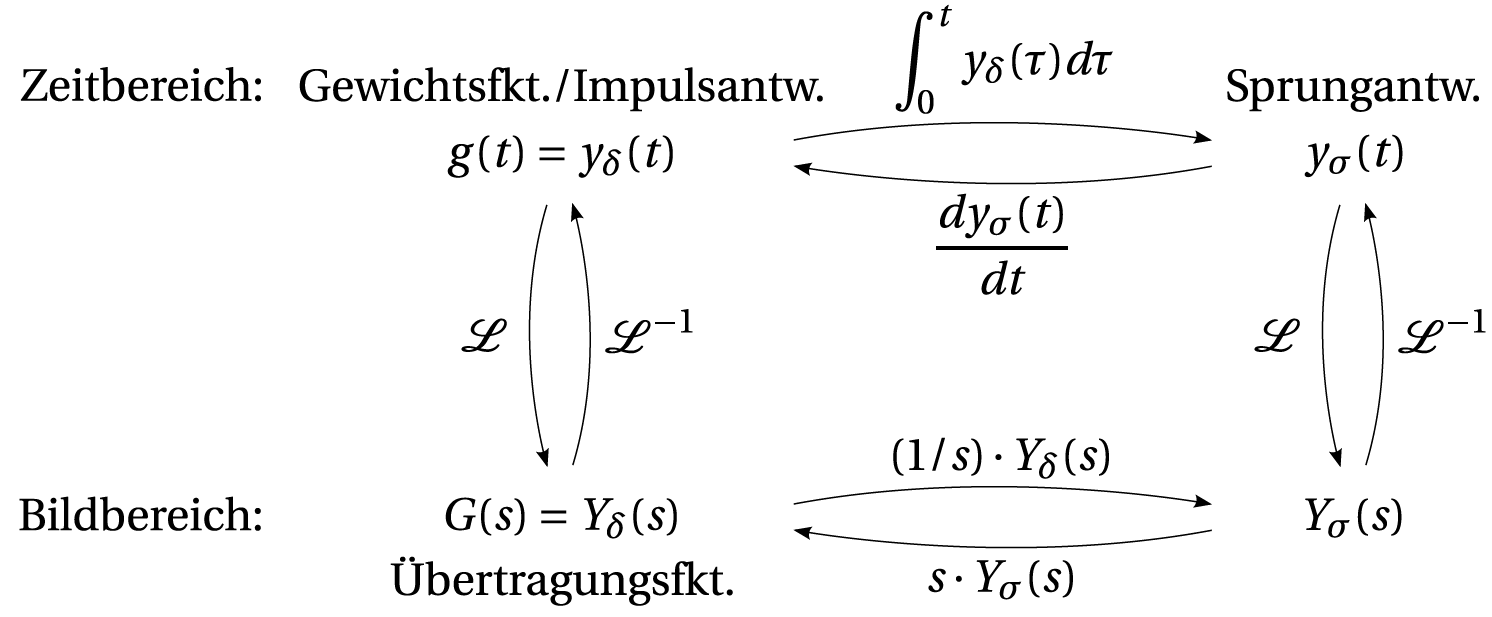
\includegraphics[width=0.75\columnwidth]{images/impulsantwort_uebertragungsfunktion.png} 
\end{center}


\subsubsection{Übertragungsfunktion $\bm{G(s)}$ aus DGL bestimmen}

\begin{tabular}{ll}
    DGL:    & $\sum \limits_{k=0}^{n} a_k \cdot y^{(k)} (t) = f(t) = \sum \limits_{k=0}^{m} b_k \cdot x^{(k)} (t)$ \\
    UTF:    & $G(s) = \frac{q(s)}{p(s)} = \frac{\sum \limits_{k=0}^{m} b_k \cdot s^k}{\sum \limits_{k=0}^{n} a_k \cdot s^k}$ 
\end{tabular}

$$ \underrightarrow{f(t) = x(t)} \quad G(s) = \frac{1}{p(s)} = \frac{1}{\sum \limits_{k=0}^{n} a_k \cdot s^k} = \frac{1}{\text{char. \; Polynom}} $$



\subsection[Übertragungsfunktion -- Frequenzgang]{Übertragungsfunktion $\bm{G(s)}$ \textrightarrow\ Frequenzgang $\bm{H(\omega)}$}

Wenn die Konvergenzhalbebene einer Übertragungsfunktion $G(s)$ eines LTI-Systems die \textbf{imaginäre Achse beinhaltet}, so gilt:

$$ H(\omega) = G(j \omega) = G(s) \biggr|_{s = j \omega} \qquad \text{\textrightarrow\ in $G(s)$ alle $s$ durch $\jimg \omega$ ersetzen} $$


\subsection{BIBO-Stabilität}

Ein LTI-System ist BIBO-stabil, wenn ein \textbf{beschränktes Eingangssignal} $x(t)$ zu einem \textbf{beschränkten Ausgangssignal} $y(t)$
mit $\mathrm{max}( \vert y(t) \vert) < \infty$ führt.


\subsubsection{Zeitbereich}

Ein LTI-System ist BIBO-stabil, wenn die Impulsantwort \textbf{absolut integrierbar} ist:
$$ \int \limits_{- \infty}^{\infty} \vert y_{\delta} (t) \vert \, \diff t = \int \limits_{-\infty}^{\infty} \vert g(t) \vert \, \diff t < \infty $$


\subsubsection{Bildbereich}

Ein LTI-System ist BIBO-stabil, wenn  die \textbf{Konvergenzhalbebene} der Übertragungsfuntion $G(s)$ die \textbf{imaginäre Achse enthält}

\textrightarrow\ $\Re(s_p) < 0$ bzw. Realteil der Polstelle $< 0$


\subsection{Pol-Nullstellen Plan (PN-Plan)}

Der PN-Plan stellt die Polstellen und Nullstellen einer Übertragungsfunktion $G(s)$ eines LTI-Systems in der \textbf{komplexen Zahlenebene} dar.

\vspace{0.2cm}

\begin{tabular}{ll}
    Nullstellen:    & als Kreise dargestellt    \\
    Polstellen:     & als Kreuzchen dargestellt 
\end{tabular}


\subsection{Zusammengesetzte LTI-Systeme}

\begin{tabular}{ccc}
    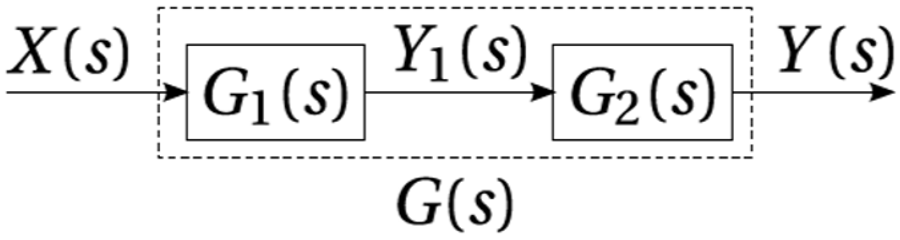
\includegraphics[width=3.5cm]{images/zusammengesetzte_LTI-systeme_a.png}    & & 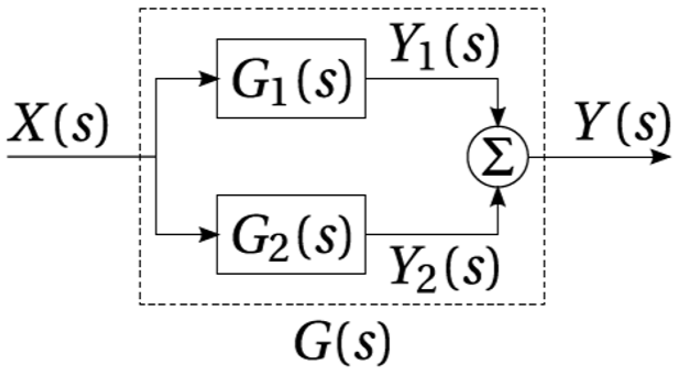
\includegraphics[width=3.5cm]{images/zusammengesetzte_LTI-systeme_b.png}    \\
    $G(s) = G_1(s) \cdot G_2(s)$                                                & & $G(s) = G_1(s) + G_2(s)$                                                    \\
    \\
    \\
    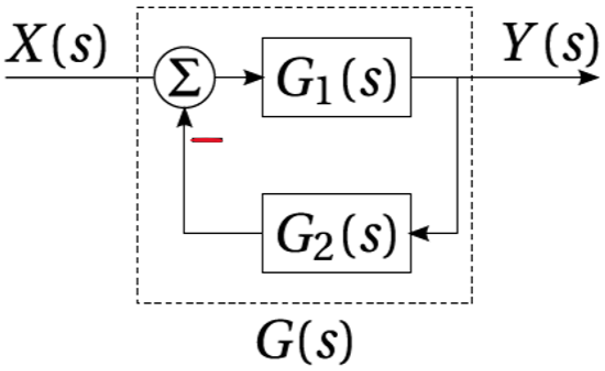
\includegraphics[width=3.5cm]{images/zusammengesetzte_LTI-systeme_c.png}    & & 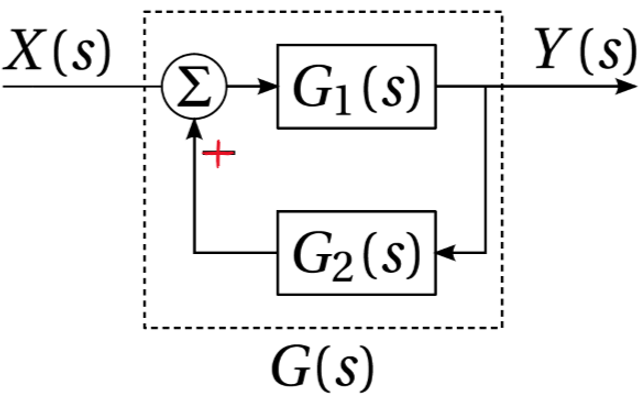
\includegraphics[width=4cm]{images/zusammengesetzte_LTI-systeme_d.png}      \\
    $G(s) = \frac{G_1(s)}{1 + G_1(s) \cdot G_2(s)}$                             & & $G(s) = \frac{G_1(s)}{1 - G_1(s) \cdot G_2(s)}$
\end{tabular}


		\section{Mathematische Grundlagen}

\subsection{Trigonometrie}

% 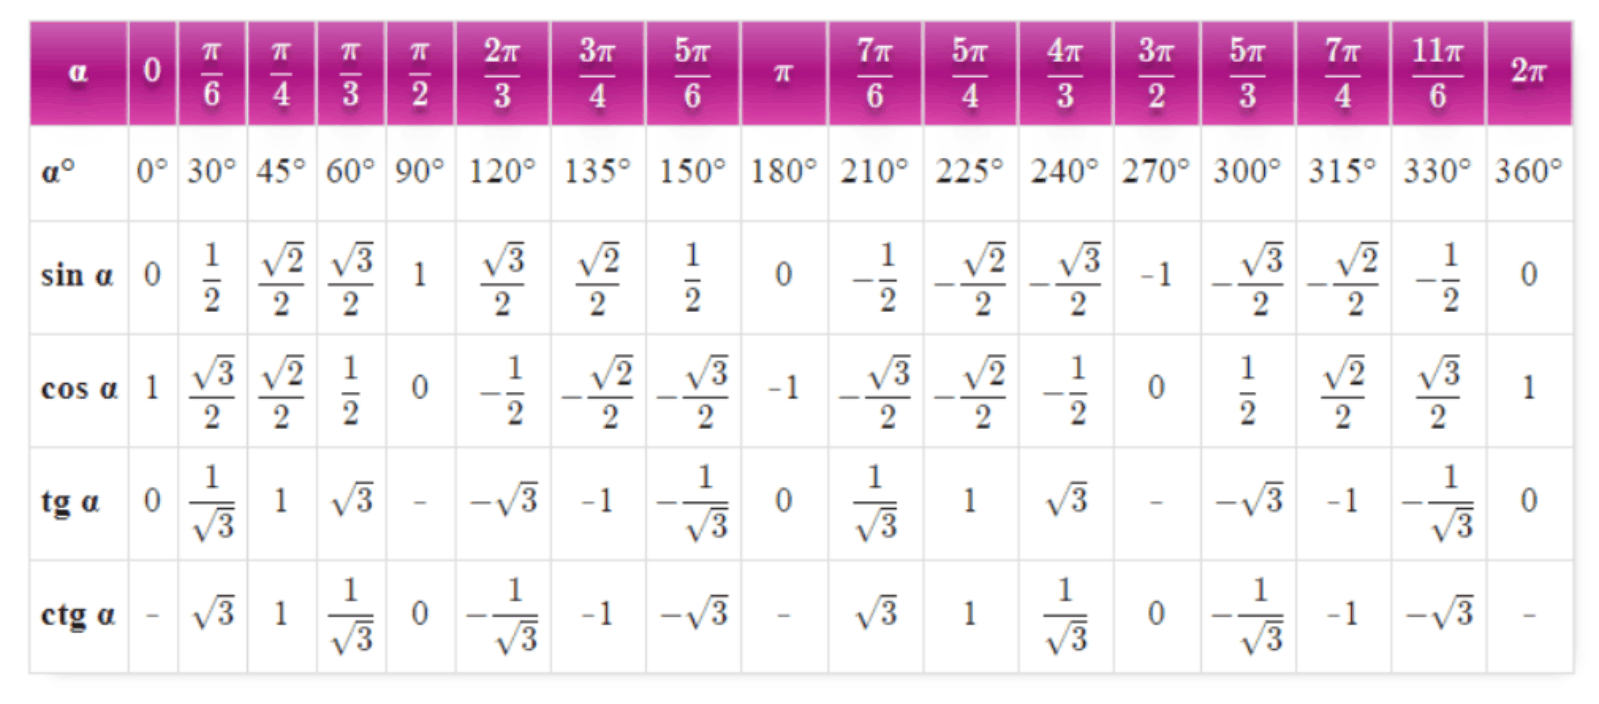
\includegraphics[width=\columnwidth]{images/trigo.png}

\begingroup
\renewcommand{\arraystretch}{2}
\setlength{\tabcolsep}{0mm}
\scalebox{0.33}{
\Huge
\begin{tabularx}{3\columnwidth}{rp{1mm}V{3}*{17}{C}}
    \rowcolor{subsectioncolor!30}$\bm{\alpha}$\phantom{${}^{\circ}$} && $0$ & $\dfrac{\pi}{6\mathstrut}$ & $\dfrac{\pi}{4}$ & $\dfrac{\pi}{3}$ & $\dfrac{\pi}{2}$ & $\dfrac{2\pi}{3}$ & $\dfrac{3\pi}{4}$ & $\dfrac{5\pi}{6}$ & $\pi$ & $\dfrac{7\pi}{6}$ & $\dfrac{5\pi}{4}$ & $\dfrac{4\pi}{3}$ & $\dfrac{3\pi}{2}$ & $\dfrac{5\pi}{3}$ & $\dfrac{7\pi}{4}$ & $\dfrac{11\pi}{6}$ & $2\pi$ \\\hline
    \rowcolor{subsectioncolor!30}$\bm{\alpha^\circ}$ && \phantom{${}^\circ$}$0^\circ$ & $30^\circ$ & $45^\circ$ & $60^\circ$ & $90^\circ$ & $120^\circ$ & $135^\circ$ & $150^\circ$ & $180^\circ$ & $210^\circ$ & $225^\circ$ & $240^\circ$ & $270^\circ$ & $300^\circ$ & $315^\circ$ & $330^\circ$ & $360^\circ$ \\\hline
    $\bm{\sin(\alpha)}$ && $0$ & $\dfrac{1}{2\mathstrut}$ & $\dfrac{\sqrt{2}}{2}$ & $\dfrac{\sqrt{3}}{2}$ & $1$ & $\dfrac{\sqrt{3}}{2}$ & $\dfrac{\sqrt{2}}{2}$ & $\dfrac{1}{2}$ & $0$ & $-\dfrac{1}{2}$ & $-\dfrac{\sqrt{2}}{2}$ & $-\dfrac{\sqrt{3}}{2}$ & $-1$ & $-\dfrac{\sqrt{3}}{2}$ & $-\dfrac{\sqrt{2}}{2}$ & $-\dfrac{1}{2}$ & $0$ \\\hline
    $\bm{\cos(\alpha)}$ && $1$ & $\dfrac{\sqrt{3}}{2\mathstrut}$ & $\dfrac{\sqrt{2}}{2}$ & $\dfrac{1}{2}$ & $0$ & $-\dfrac{1}{2}$ & $-\dfrac{\sqrt{2}}{2}$ & $-\dfrac{\sqrt{3}}{2}$ & $-1$ & $-\dfrac{\sqrt{3}}{2}$ & $-\dfrac{\sqrt{2}}{2}$ & $-\dfrac{1}{2}$ & $0$ & $\dfrac{1}{2}$ & $\dfrac{\sqrt{2}}{2}$ & $\dfrac{\sqrt{3}}{2}$ & $1$ \\\hline
    $\bm{\tan(\alpha)}$ && $0$ & $\dfrac{\sqrt{3}}{3\mathstrut}$ & $1$ & $\sqrt{3}$ & $\pm\infty$ & $-\sqrt{3}$ & $-1$ & $-\dfrac{\sqrt{3}}{3}$ & $0$ & $\dfrac{\sqrt{3}}{3}$ & $1$ & $\sqrt{3}$ & $\pm\infty$ & $-\sqrt{3}$ & $-1$ & $-\dfrac{\sqrt{3}}{3}$ & $0$ \\\hline
    $\bm{\cot(\alpha)}$ && $\pm\infty$ & $\sqrt{3}$ & $1$ & $\dfrac{\sqrt{3}}{3\mathstrut}$ & $0$ & $-\dfrac{\sqrt{3}}{3}$ & $-1$ & $-\sqrt{3}$ & $\pm\infty$ & $\sqrt{3}$ & $1$ & $\dfrac{\sqrt{3}}{3}$ & $0$ & $-\dfrac{\sqrt{3}}{3}$ & $-1$ & $-\sqrt{3}$ & $\pm\infty$ \\
\end{tabularx}}
\endgroup


\subsubsection{Beziehungen zwischen $\bm{\sin(x)}$ und $\bm{\cos(x)}$}

\renewcommand{\arraystretch}{1.3}
\begin{tabular}{ll}
    $\sin(-a) = -\sin(a)$                                           & $\cos(-a) = \cos(a)$                                              \\
    $\sin(\pi - a) = \sin(a)$                                       & $\cos(\pi -a) = - \cos(a)$                                        \\		
    $\sin(\pi + a) = -\sin(a)$                                      & $\cos(\pi + a) = - \cos(a)$                                       \\	
    $\sin(\frac{\pi}{2} - a) = \sin(\frac{\pi}{2} + a) = \cos(a)$   & $\cos(\frac{\pi}{2} - a) = - \cos(\frac{\pi}{2} + a) = \sin(a)$
\end{tabular}


\subsubsection{Additionstheoreme}

\begin{tabular}{l}
    $\sin(a \pm b) = \sin(a) \cdot \cos(b) \pm \cos(a) \cdot \sin(b)$           \\
    $\cos(a \pm b) = \cos(a) \cdot \cos(b) \mp \sin(a) \cdot \sin(b) $          \\
    $\tan(a \pm b) = \frac{\tan(a) \pm \tan(b)}{1 \mp \tan(a) \cdot \tan(b)}$
\end{tabular}


\subsubsection{Summen und Differenzen}

\begin{tabular}{l}
    $\sin(a) + \sin(b) = 2 \cdot \sin \big( \frac{a+b}{2} \big) \cdot \cos \big( \frac{a-b}{2} \big)$   \\
    $\sin(a) - \sin(b) = 2 \cdot \sin \big( \frac{a-b}{2} \big) \cdot \cos \big( \frac{a+b}{2} \big)$   \\
    $\cos(a) + \cos(b) = 2 \cdot \cos \big( \frac{a+b}{2} \big) \cdot \cos \big( \frac{a-b}{2} \big)$   \\
    $\cos(a) - \cos(b) = -2 \cdot \sin \big( \frac{a+b}{2} \big) \cdot \sin \big( \frac{a-b}{2} \big)$  \\
    $\tan(a) \pm \tan(b) = \frac{\sin(a \pm b)}{\cos(a) \cdot \cos(b)}$ 
\end{tabular}


\subsubsection{Produkte}

\begin{tabular}{l}
    $\sin(a) \cdot \sin(b) = \frac{1}{2} \big( \cos(a-b) - \cos(a+b) \big) $    \\
    $\cos(a) \cdot \cos(b) = \frac{1}{2} \big( \cos(a-b) + \cos(a+b) \big) $    \\	
    $\sin(a) \cdot \cos(b) = \frac{1}{2} \big( \sin(a-b) + \sin(a+b) \big) $ 
\end{tabular}

    
\subsubsection{Winkelvielfache und Halbwinkel}

\begin{tabular}{ll}
    $\sin(2a) = 2 \, \sin(a) \cdot \cos(a)$                                 & $\sin(3a) = 3 \, \sin(a) -4 \, \sin^3(a)$                                 \\
    $\sin(4a) = 8 \, \cos^3(a) \cdot \sin(a) - 4 \, \cos(a) \cdot \sin(a)$  & $\sin \big( \frac{a}{2} \big) = \sqrt{\frac{1}{2}(1-\cos(a))}$            \\
    \\
    $\cos(2a) = \cos^2(a) - \sin^2(a)$                                      & $\cos(3a) = 4 \, \cos^3(a) -3 \, \cos(a)$                                 \\
    $\cos(4a) = 8 \, \cos^4(a) - 8 \, \cos^2(a) + 1$                        & $\cos \big( \frac{a}{2} \big) = \sqrt{\frac{1}{2}(1+\cos(a))}$
\end{tabular}


\subsubsection{Potenzen}

\begin{tabular}{ll}
    $\sin^2(a) = \frac{1}{2}(1-\cos(2a))$                   & $\cos^2(a) = \frac{1}{2}(1+\cos(2a))$                 \\	
    $\sin^3(a) = \frac{1}{4}(3\, \sin(a) - \sin(3a))$       & $\cos^3(a) = \frac{1}{4}(\cos(3a) + 3 \, \cos(a)$     \\	
    $\sin^4(a) = \frac{1}{8}(\cos(4a) -4 \, \cos(2a) +3)$   & $\cos^4(a) = \frac{1}{8}(\cos(4a) +4 \, \cos(2a) +3)$ 	
\end{tabular}

\subsection{Komplexwertige Exponentialfunktion}

\subsubsection{Exponentialgesetze}

Die Exponentialgesetze bleiben in $\mathbb{C}$ für \myul{\textbf{ganzzahlige}} Exponenten erhalten!

\begin{tabular}{lll ll}
    $\e^a \cdot \e^b = \e^{a+b}$    & & $\e^a : \e^b = \e^{a-b}$    & & $a, \; b \in \mathbb{C}$    \\
    $(\e^a)^k = \e^{ka}$            & &                             & & $k \in \mathbb{Z}$
\end{tabular}


\subsubsection{Definition komplexwertige Exponentialfunktion}

\vspace{-0.2cm}
$$\crd{\e^z} = \e^{z_1 + jz_2} = \e^{z_1} \cdot \e^{j z_2} = \e^{z_1} \cdot \cjs(z_2)$$
Die koplexwertige Exponentialfunktion ist $2 \pi \jimg$-periodisch auf der $y$-Achse) 
    


\subsection{Partielle Integration}

\vspace{-0.2cm}
\begin{minipage}[c]{0.48\columnwidth}
    $$ \int f' \cdot g \, \diff x = f \cdot g - \int f \cdot g' \, \diff x $$
\end{minipage}
\hfill
\begin{minipage}[c]{0.48\columnwidth}
    $$ \int f \cdot g' \, \diff x  = f \cdot g - \int f' \cdot g \, \diff x $$
\end{minipage}


\subsection{Wichtige Ableitungen / Integrale}

\renewcommand{\arraystretch}{2}
\begin{tabular}{| c | c | c | c |}
    \hline
    $\bm{f'(t)}$                                                & $\bm{f(t)}$                           & $\bm{F(t)}$                   &               \\
    \hline
    $n \cdot \cos(n \, t)$                                      & $\sin(n \, t)$                        & $- \frac{\cos(n \, t)}{n}$    & $(n \neq 0)$  \\
    \hline     
    $- n \cdot \sin(n \, t)$                                    & $\cos(n \, t)$                        & $ \frac{\sin(n \, t)}{n}$     & $(n \neq 0)$  \\
    \hline
    \cbl{$ - \jimg \, \omega \, \e^{- \jimg \, \omega \, t}$}   & \cbl{$\e^{- \jimg \, \omega \, t}$}   & \cbl{$\frac{\e^{- \jimg \, \omega \, t}}{- \jimg \, \omega} = \frac{\jimg}{\omega} \e^{-\jimg \, \omega \, t}$} & \cbl{ $(n \neq 0)$ } \\
    \hline
\end{tabular}
\renewcommand{\arraystretch}{1}


\subsection[Einheitsprungfunktion ]{Einheitsprungfunktion $\sigma(t)$}

\begin{minipage}[c]{0.38\columnwidth}
    $$\sigma(t) = \begin{cases}			
    0           & \text{für} \; t < 0 \\
    \frac{1}{2} & \text{für} \; t = 0 \\ 
    1           & \text{für} \; t > 0 
\end{cases}$$
\end{minipage}
\hfill
\begin{minipage}[c]{0.5\columnwidth}
    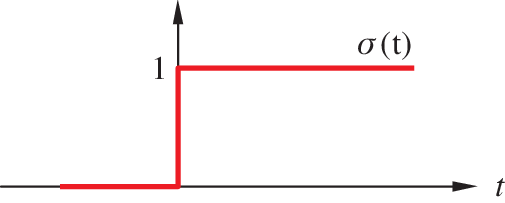
\includegraphics[width=\columnwidth]{images/einheitssprung.png}
\end{minipage}


\subsection{Polynomdivision}

Liefert Summe aus ganzrationaler Funktion und echt gebrochener Funktion.


\example{Polynomdivision}

\polylongdiv[style=C]{-2x^2-x-1}{x-1} 
    
    
\subsection{Partialbruchzerlegung}

\begin{tabular}{lll}
    (1)     & echt gebrochen ($m < n$)  \\
            & Ja: \textrightarrow\ (2)   & Nein: Polynomdivision \\
    (2)     & Nenner faktorisieren      \\
            & pro Faktor ein Teilbruch  \\
    (3)     & Berechnung Zählerkonstanten       \\
    (3.1)   & Gleichnahmig machen (kgV) \\
    (3.2)   & Zählergleichung           \\
    (3.3)   & Einsetzen von 'guten' $x$-Werten  \\			
\end{tabular}


\example{Partialbruchzerlegung}

\renewcommand{\arraystretch}{1.7}
\begin{tabular}{ll}
(1)     & $f(x) = \frac{1}{a^2 - x^2}$                                  \\
(2)     & $a^2 - x^2 = (a+x)(a-x)$                                      \\
(3)     & $\frac{A}{a+x} + \frac{B}{a-x} = \frac{1}{a^2 - x^2}$         \\
(3.1)   & $\frac{A(a-x) + B(a+x)}{a^2 - x^2} = \frac{1}{a^2 - x^2}$     \\
(3.2)   & $A(a-x) + B(a+x) = 1$                                         \\
(3.3)   & $x = a$ \textrightarrow\ $B(2a) = 1$ \textrightarrow\ $B = \frac{1}{2a}$    \\			
        & $x = -a$ \textrightarrow\ $A(2a) = 1$ \textrightarrow\ $A = \frac{1}{2a}$
\end{tabular}


\subsubsection{Spezielle Ansätze PBZ}

\renewcommand{\arraystretch}{2}
\begin{tabular}{ll}
    $f(x)$  & $ = \frac{5x^2-37x+54}{x^3-6x^2+9x} = \frac{A}{x}+\frac{B}{x-3}+\frac{C}{(x-3)^2} = \frac{A(x-3)^2+Bx(x-3)+Cx}{x(x-3)^2}$ \\ 
    $f(x)$  & $ = \frac{1.5x}{x^3-6x^2+12x-8} = \frac{A}{x-2}+\frac{B}{(x-2)^2}+\frac{C}{(x-2)^3 } =\frac{A(x-2)^2+B(x-2)+C}{(x-2)^3}$  \\
    $f(x)$  & $ = \frac{x^2-1}{x^3+2x^2-2x-12} = \frac{A}{x-2}+\frac{Bx+C}{x^2+4x+6} = \frac{A(x^2+4x+6)+(Bx+C)(x-2)}{(x-2)(x^2+4x+6)}$
\end{tabular}
\renewcommand{\arraystretch}{1}


    \end{layout}
\end{document}
